\documentclass{article}
\usepackage[utf8]{inputenc}
\usepackage[a4paper,top=2cm,bottom=2cm,left=3cm,right=3cm,marginparwidth=1.75cm]{geometry}
\usepackage{amsmath}
\usepackage{graphicx}
\usepackage[colorlinks=true, allcolors=blue]{hyperref}

\begin{document}

\begin{titlepage}

\center % Center everything on the page

\newcommand{\HRule}{\rule{\linewidth}{0.4mm}} % Barra horizontal

\begin{figure}[h]
    \centering
    
\includegraphics[width=0.24\linewidth]{images/uniMinho.jpg}
\end{figure}

%\textsc{\Large Universidade do Minho}\\[0.75cm]  % Name of your university/college
\textsc{\Large Licenciatura em Ciências da Computação}\\[0.4cm] % Nome do curso
\textsc{\Large Sistemas de Comunicações e Redes}\\[5cm]

{\Large\bfseries Ensaio Escrito}\\[0.5cm]
%{\huge \bfseries Pesquisa sobre \textit{frameworks} de separação de camadas} % Título
{\LARGE \bfseries   Nível de Ligação Lógica - Ethernet e Protocolo ARP; Redes Sem Fios (IEEE 802.11)} % Título


\vspace{5cm} % Autores
{\bfseries Grupo 28} \\ \vspace{3mm}
Davide Santos (A102938) \\ \vspace{3mm}
Edgar Araújo (A102946) \\ \vspace{3mm}
Pedro Augusto Camargo (A102504) \\ \vspace{3mm}
\vspace{0.2cm}
{Outubro 2023}\\[0.2cm] % Data

\vfill % Fill the rest of the page with whitespace
\end{titlepage}

\tableofcontents
\pagebreak

\section{Captura e Análise de Tramas Ethernet}
\subsection*{Selecione a trama Ethernet que contém a mensagem HTTP GET.}

\begin{verbatim}
    No. Time Source Destination Protocol Length Info
    309579 222.320604325 192.168.1.39 193.136.9.240 HTTP 175 GET /
    ferramentas/CORE/xubuncore.html HTTP/1.1

    Frame 309579: 175 bytes on wire (1400 bits), 175 bytes captured (1400 bits) 
    on interface wlp3s0, id 0

    Ethernet II, Src: CloudNet_c9:c9:03 (30:03:c8:c9:c9:03), Dst: Sagemcom_9f:a6:37
    (10:d7:b0:9f:a6:37)

    Internet Protocol Version 4, Src: 192.168.1.39, Dst: 193.136.9.240

    Transmission Control Protocol, Src Port: 56218, Dst Port: 80, Seq: 1, Ack: 1, 
    Len: 109

    Hypertext Transfer Protocol
\end{verbatim}

\subsection{Anote os endereços Ethernet (ou MAC) de origem e de destino da trama
capturada com o pedido HTTP. Identifique a que sistemas se referem. Justifique.}

Os endereços Ethernet localizam-se na camada Ethernet do modelo OSI, e são:
\begin{itemize}
    \item Endereço de origem: 30:03:c8:c9:c9:03 (CloudNet\_c9:c9:03 / O nosso computador) \linebreak
    O endereço de origem é o endereço do nosso computador, pois foi o computador que enviou a trama.
    \item Endereço de destino: 10:d7:b0:9f:a6:37 (Sagemcom\_9f:a6:37 / O router) \linebreak
    O endereço de destino é o endereço do router, pois foi o router que recebeu a trama.
\end{itemize}

\subsection{Analisando os campos do cabeçalho da trama capturada, diga, justificando, qual
o protocolo encapasulado nessa trama.}

O protocolo encapasulado é o IPv4, pois o campo Type da trama tem o valor 0x0800, que corresponde ao protocolo IPv4.

\begin{figure}[h]
    \centering
    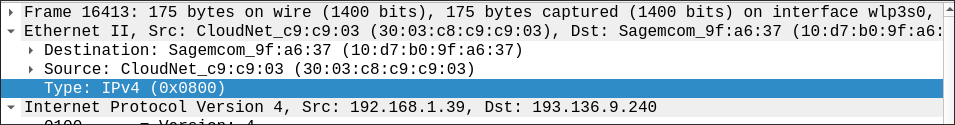
\includegraphics[width=0.8\textwidth]{images/type.png}
    \caption{\label{fig:type}Campo Type da trama.}
\end{figure}

\subsection{Quantos bytes são usados desde o início da trama até ao caractere ASCII “G” do
método HTTP GET? Calcule e indique, em percentagem, a sobrecarga (overhead)
introduzida pela pilha protocolar no envio do HTTP GET (considere os bytes
ocupados pela camada física e pelo FCS, indicados na Figura 1).}

\begin{figure}[h]
    \centering
    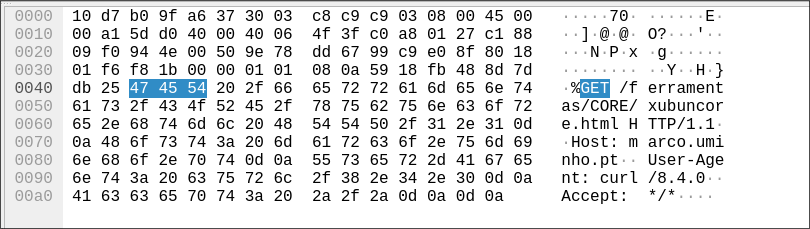
\includegraphics[width=0.8\textwidth]{images/byte.png}
    \caption{\label{fig:byte}Trama em formato de bytes.}
\end{figure}
ain.
\begin{figure}[h]
    \centering
    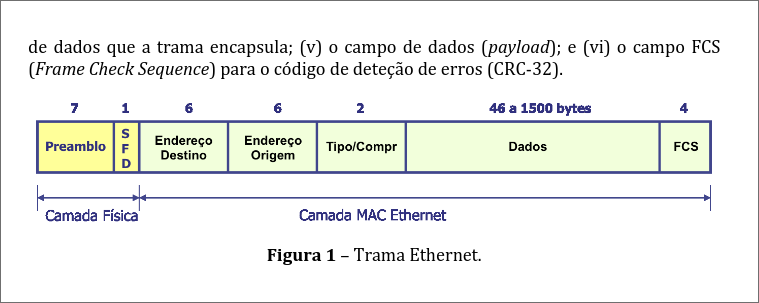
\includegraphics[width=0.8\textwidth]{images/fcs.png}
    \caption{\label{fig:fcs}Tamanhos do preamblo, SFD e FCS.}
\end{figure}

Observa-se que o caractere "G" está na posição 0x42 da trama = 66 bytes. Considerando que o preamblo e o SFD ocupam 7+1 bytes no inicio da trama, o numero de bytes usados desde o incio da trama ate ao caractere ASCII "G" é 66+8 = 74 bytes.

O tamanho da trama, sem o preamblo, o SFD, e o FCS é 175 bytes, com o preamblo, o SFD, e o FCS é 175+7+1+4 = 187 bytes.
O tamanho do HTTP GET é 175-66=109 bytes. Logo, a sobrecarga é de 187-109=78 bytes.
Em percentagem temos: 78/187 = 41.71\% de sobrecarga.

\subsection*{A seguir responda às seguintes perguntas, baseado no conteúdo da trama Ethernet que
contém o primeiro byte da resposta HTTP}

\begin{verbatim}
    No. Time Source Destination Protocol Length Info
    16427 13.899293562 193.136.9.240 192.168.1.39 HTTP 479 HTTP/1.1 200 OK(text/html)

    Frame 16427: 479 bytes on wire (3832 bits), 479 bytes captured (3832 bits) on interface wlp3s0, id0

    Ethernet II, Src: Sagemcom_9f:a6:37 (10:d7:b0:9f:a6:37), Dst: CloudNet_c9:c9:03
    (30:03:c8:c9:c9:03)
    Destination: CloudNet_c9:c9:03 (30:03:c8:c9:c9:03)
    Source: Sagemcom_9f:a6:37 (10:d7:b0:9f:a6:37)
    Type: IPv4 (0x0800)

    Internet Protocol Version 4, Src: 193.136.9.240, Dst: 192.168.1.39
    0100 .... = Version: 4
    .... 0101 = Header Length: 20 bytes (5)
    Differentiated Services Field: 0x00 (DSCP: CS0, ECN: Not-ECT)
    Total Length: 465
    Identification: 0xb880 (47232)
    010. .... = Flags: 0x2, Don't fragment
    ...0 0000 0000 0000 = Fragment Offset: 0
    Time to Live: 53

    Protocol: TCP (6)
    Header Checksum: 0xfe5e [validation disabled]
    [Header checksum status: Unverified]
    Source Address: 193.136.9.240
    Destination Address: 192.168.1.39
    Transmission Control Protocol, Src Port: 80, Dst Port: 37966, Seq: 8689, Ack: 110, Len: 413
    [7 Reassembled TCP Segments (9101 bytes): #16415(1448), #16417(1448), #16419(1448), #16421(1448),
    #16423(1448), #16425(1448), #16427(413)]

    Hypertext Transfer Protocol
    Line-based text data: text/html (245 lines)
\end{verbatim}

\subsection{Quais são os endereços Ethernet da origem e destino? A que sistemas de rede
correspondem? Justifique.}

Os endereços Ethernet localizam-se na camada Ethernet do modelo OSI, e são:
\begin{itemize}
    \item Endereço de origem: 10:d7:b0:9f:a6:37 (Sagemcom\_9f:a6:37 / O router) \linebreak
    O endereço de origem é o endereço do router, pois foi o router que enviou a trama.
    \item Endereço de destino: 30:03:c8:c9:c9:03 (CloudNet\_c9:c9:03 / O nosso computador) \linebreak
    O endereço de destino é o endereço do nosso computador, pois foi o nosso computador que recebeu a trama.
\end{itemize}

\subsection{Atendendo ao conceito de desencapsulamento protocolar, identifique os vários
protocolos contidos na trama recebida.}

Os protocolos contidos na trama recebida são:
\begin{itemize}
    \item Ethernet II
    \item IPv4
    \item TCP
    \item HTTP
\end{itemize}

\section{Protocolo ARP}
\subsection*{Selecione um host (PC, servidor) de um departamento à sua escolha. Neste host inicie a
captura de tráfego com o Wireshark do CORE. A partir desse host efectue pings para dois
hosts localizados na rede do outro departamento. Pare a captura de tráfego no
Wireshark e localize o tráfego ARP, usando o filtro arp.}

\begin{figure} [h]
    \centering
    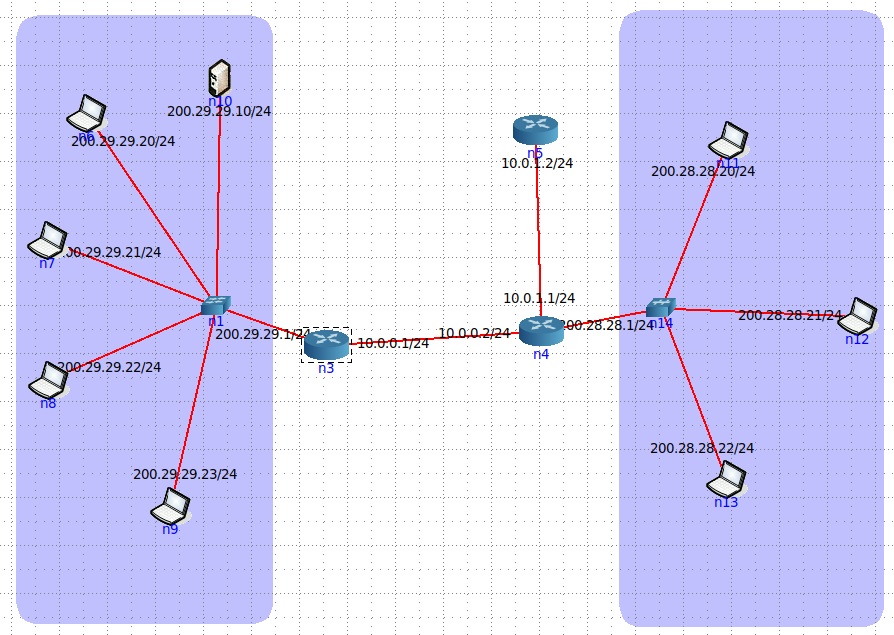
\includegraphics[width=0.8\linewidth]{ligacoes-routers.png}
    \caption{Rede}
    \label{fig:enter-label}
\end{figure}

\subsection{Abra uma consola no host onde efetou o ping. Observe o conteúdo da tabela ARP com o comando arp.}

\begin{figure} [h]
    \centering
    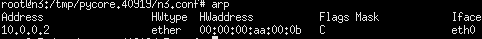
\includegraphics[width=1\linewidth]{dois-pings-tabela-arp.png}
    \caption{Enter Caption}
    \label{fig:enter-label}
\end{figure}

\subsubsection{Com a ajuda do manual arp (man arp), interprete sucintamente o significado de cada uma das colunas da tabela.}

\textbf{Address}: O endereço IP associado ao endereço MAC.

\textbf{HWtype}: O tipo de hardware, que é "ether" neste caso, indicando Ethernet.

\textbf{HWaddress}: O endereço MAC associado ao endereço IP.

\textbf{Flags}: As bandeiras indicam o estado da entrada na tabela. "C" significa que a entrada está completa, ou seja, o mapeamento IP-MAC é conhecido e válido.

\textbf{Mask}: Se estiver preenchido, indica uma máscara de sub-rede associada ao endereço IP.

\textbf{Iface}: A interface de rede à qual o endereço MAC está associado.\newline

Neste caso, com base na tabela ARP, existe apenas uma entrada:

\textbf{Endereço IP 10.0.0.2} está associado ao \textbf{endereço MAC 00:00:00:aa:00:0b}. A entrada na tabela ARP está marcada como completa (C) e associada à interface \textbf{eth0}.

Essa entrada significa que o endereço IP 10.0.0.2 está associado ao endereço MAC 00:00:00:aa:00:0b e que essa associação é conhecida e válida. Portanto, o sistema já possui essa informação na tabela ARP e não precisa fazer solicitações ARP adicionais para esse endereço, pois já tem o mapeamento IP-MAC correspondente.

\subsubsection{Indique, justificando, qual o equipamento da rede em questão que poderá apresentar a maior tabela ARP em termos de número de entradas.}

Na rede, o equipamento que provavelente apresenta um maior número de entradas na tabela ARP será, provavelmente, o router n3, uma vez que apresenta 6 ligações, ao invés do n4 que apresenta 5 ligações.

\subsubsection{Realize as operações necessárias para completar a tabela ARP identificada na alínea anterior. Indique como procedeu e apresente essa tabela completa.}

Para chegar a esta tabela ARP, é necessário dar \textit{ping} a todos os dispositivos ligados ao router n3 pelo terminal e, de seguida, é deve abrir outro terminal pelo router n3 e abrir a tabela arp, chegando a um resultado semelhante ao aqui mostrado.

\begin{figure} [h]
    \centering
    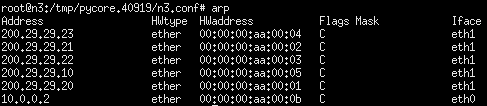
\includegraphics[width=1\linewidth]{tabela-arp-n3.png}
    \caption{Tabela ARP do router n3}
    \label{fig:enter-label}
\end{figure}

\subsection{Qual é o valor hexadecimal dos endereços origem e destino na trama Ethernet que contém a mensagem com o pedido ARP (ARP Request)? Como interpreta e justifica o endereço destino usado?}

\begin{figure} [h]
    \centering
    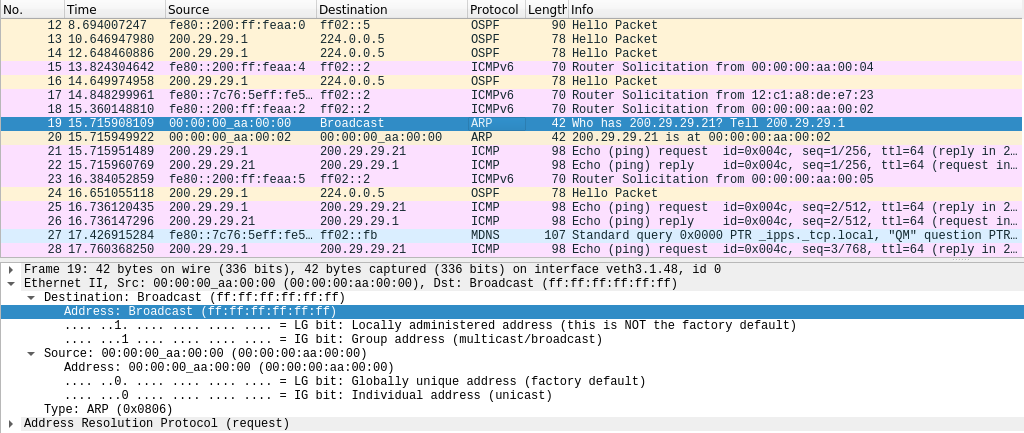
\includegraphics[width=1\linewidth]{arp-request-1.png}
    \caption{ARP Request}
    \label{fig:enter-label}
\end{figure}

O endereço de origem na trama Ethernet é 00:00:00:aa:00:00 e o endereço do destino é ff:ff:ff:ff:ff:ff. O endereço de Destino é um endereço de broadcast. Isto significa que a trama ARP está a ser enviada para todos os dispositivos na rede local para que o dispositivo de destino a reconheça. 

\subsection{Qual o valor hexadecimal no campo Tipo da trama Ethernet? O que indica?}


\begin{figure} [h]
    \centering
    
\includegraphics[width=0.5\linewidth]{tipo-arp-request.png}
    \caption{Enter Caption}
    \label{fig:enter-label}
\end{figure}

O valor hexadecimal no campo Tipo da trama Ethernet indica o tipo de dados que a trama contém. No caso de uma trama ARP, esse valor é 0x0806, que representa o protocolo ARP, como mostra a print tirada do wireshark.

\subsection{Observando a mensagem ARP, como pode saber que se trata efetivamente de um pedido ARP? Identifique o tipo de endereços contidos na mensagem ARP.}

É possível saber que se trata de um pedido ARP se observarmos o valor do campo "Opcode" (código de operação) na mensagem ARP. O valor 1 neste campo indica uma solicitação ARP. Os tipos de endereços contidos na mensagem ARP são o endereço IP e o endereço MAC.

\subsection{Explicite, em linguagem comum, que tipo de pedido ou pergunta é feita pelo host de origem à rede?}

O host de origem faz uma pergunta à rede, perguntando "Quem possui o endereço IP X?". Nesse caso, o host deseja mapear um endereço IP para um endereço MAC correspondente.

O host de origem pergunta à rede "Quem é possui este endereço IP?". Neste caso, o host quer mapear um endereço IP para um endereço MAC.

\subsection{Localize a mensagem ARP que é a resposta ao pedido ARP efetuado.}

\begin{figure} [h]
    \centering
    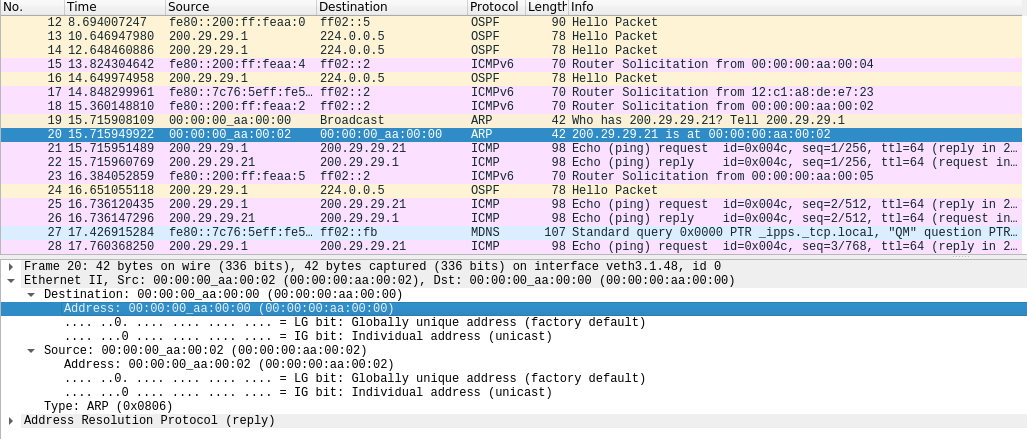
\includegraphics[width=1\linewidth]{resposta-arp-request.png}
    \caption{Mensagem ARP a responder ao pedido ARP}
    \label{fig:enter-label}
\end{figure}

A mensagem ARP em resposta ao pedido ARP está logo a seguir, como é possível ver no \textit{printscreen}.

\subsubsection{Qual o valor do campo ARP opcode? O que especifica?}

O valor do campo ARP opcode é 2, como é possível ver no \textit{printscreen} do pacote capturado pelo wireshark. Isto significa que é uma resposta ARP.

\begin{figure} [h]
    \centering
    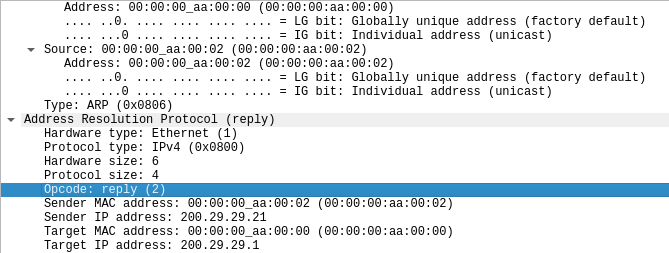
\includegraphics[width=1\linewidth]{opcode-arp-reply.png}
    \caption{ARP Opcode}
    \label{fig:enter-label}
\end{figure}

\subsubsection{Em que posição da mensagem ARP está a resposta ao pedido ARP?}

A resposta ao pedido ARP está na posição após o cabeçalho ARP (28 bytes).

\subsubsection{Justifique o modo de comunicação (unicast vs. broadcast) usado no envio da resposta ARP (ARP Reply).}

O ARP Request é enviado em \textbf{modo broadcast}, pois o host não sabe de quem é o endereço IP e precisa de perguntar a todos os dispositivos ligados quem é. A resposta ARP (ARP Reply) é enviada em \textbf{modo unicast}. Isso significa que a resposta é direcionada especificamente para o host que fez a pergunta ARP, uma vez que o dispositivo não tem necessidade de informar todos que é ele e precisa apenas de informar o host.

\subsection{Verifique se o ping feito ao segundo PC originou pacotes ARP e justifique a situação observada.}

O segundo ping feito também originou pacotes, como é possível ver no printscreen do wireshark.

\begin{figure} [h]
    \centering
    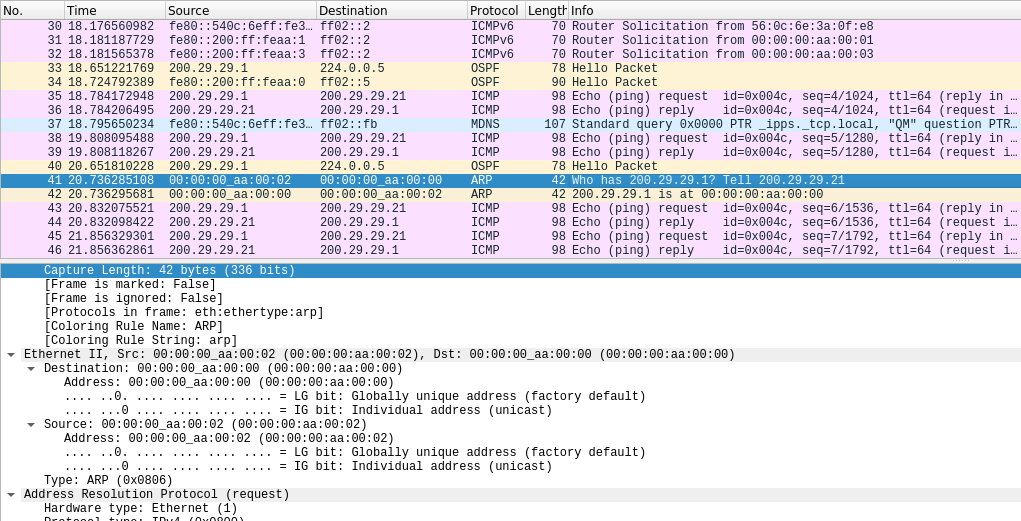
\includegraphics[width=1\linewidth]{segundo-ping-arp.png}
    \caption{Enter Caption}
    \label{fig:enter-label}
\end{figure}

\subsection{Identifique na mensagem ARP os campos que permitem definir o tipo e o tamanho dos endereços das camadas de rede e de ligação lógica que se pretendem mapear. Justifique os valores apresentados nesses campos.}

Os campos que permitem definir o tipo e o tamanho dos endereços das camadas de rede e de ligação lógica na mensagem ARP são:

\begin{itemize}
  \item \textbf{Tipo de Hardware}: Indica o tipo de hardware (geralmente Ethernet) e seu tamanho (6 bytes).
  \item \textbf{Tipo de Protocolo}: Indica o tipo de protocolo de rede (geralmente IPv4) e seu tamanho (4 bytes).
\end{itemize}


\section{Redes Sem Fios (IEEE 802.11)}
\subsection*{Acesso Rádio}
\subsection{Identifique em que frequência do espectro está a operar a rede sem fios, e o canal que corresponde essa frequência.}

\begin{figure}[h]
    \centering
    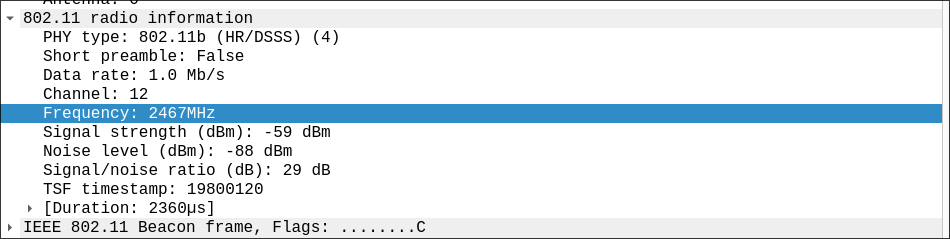
\includegraphics[width=0.8\textwidth]{images/freq.png}
    \caption{\label{fig:freq}Frequencia e channel de operacao da rede sem fios.}
\end{figure}

A rede sem fios está a operar na frequência de 2.467 GHz, e o canal que corresponde a essa frequência é o 12.

\subsection{Identifique a versão da norma IEEE 802.11 que está a ser usada.}

\begin{figure}[h]
    \centering
    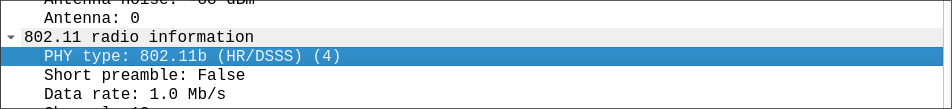
\includegraphics[width=0.8\textwidth]{images/ver.png}
    \caption{\label{fig:ver}Versao da norma IEEE 802.11, e data rate de operacao da rede sem fios.}
\end{figure}

A versao da norma IEEE 802.11 que está a ser usada é a 802.11b.

\subsection{Qual o débito a que foi enviada a trama escolhida? Será que esse débito  corresponde ao débito máximo a que a interface Wi-Fi pode operar? Justifique.}

Como pode ser observado na Figura \ref{fig:ver} o data rate de operacao da rede sem fios para a trama escolhida é de 1 Mb/s.

\begin{figure}[h]
    \centering
    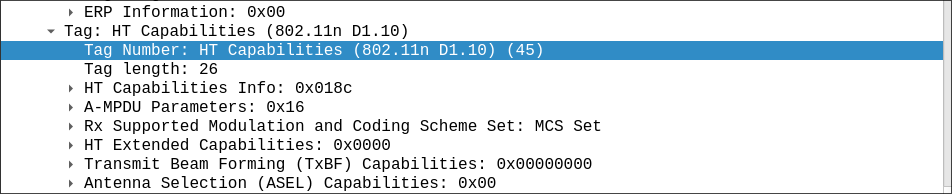
\includegraphics[width=0.8\textwidth]{images/ht.png}
    \caption{\label{fig:ht}Capacidade de operacao da rede sem fios.}
\end{figure}

\begin{figure}[h]
    \centering
    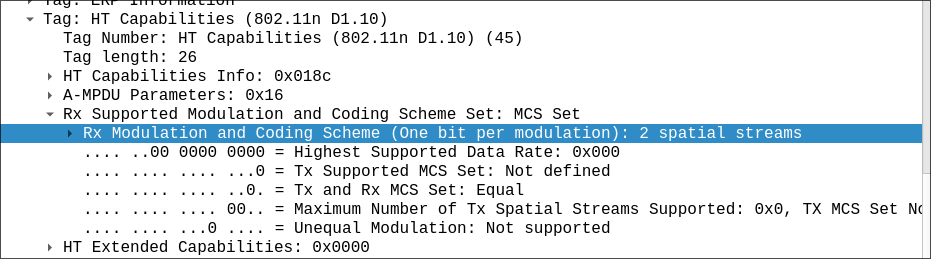
\includegraphics[width=0.8\textwidth]{images/channels.png}
    \caption{\label{fig:channels}Numero de Spatial Streams e canais de operacao da rede sem fios.}
\end{figure}

\begin{figure}[h]
    \centering
    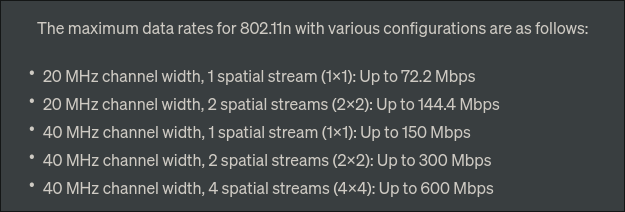
\includegraphics[width=0.8\textwidth]{images/chat.png}
    \caption{\label{fig:chat}Data rates de operacao da rede sem fios. (GPT-3.5)}
\end{figure}

De acordo com a HT Capabilities (Figura \ref{fig:ht}) a versao 802.11n é suportada, e
e de acordo com a Figura \ref{fig:channels} o numero de Spatial Streams é de 2, logo a data rate de operacao da rede sem fios pode variar de 144.4 Mbps a 300 Mbps conforme a Figura \ref{fig:chat}.

Logo o data rate de operacao da rede sem fios para a trama escolhida não corresponde ao débito máximo a que a interface Wi-Fi pode operar.

\subsection{Verifique qual a força do sinal (signal strength) e a qualidade expectável de  receção da trama, tendo em conta a tabela apresentada em Anexo.}

\begin{figure}[h]
    \centering
    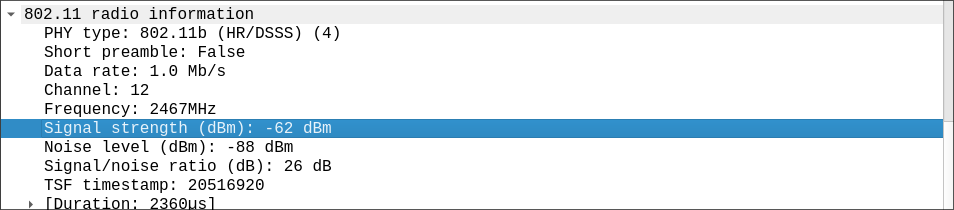
\includegraphics[width=0.8\textwidth]{images/signal.png}
    \caption{\label{fig:signal}Signal strength da trama.}
\end{figure}

De acordo com a signal strength de -62 dBm, a qualidade expectável de receção da trama é de "reliable signal strength (the edge of what is considered accurate to support Voice over WLAN)".

\subsection*{Scanning Passivo e Scanning Ativo}
\subsection{Selecione a trama beacon nr. 100+NG, sendo NG o seu número de grupo. Esta  trama pertence a que tipo de tramas 802.11? Indique o valor dos seus  identificadores de tipo e de subtipo. Em que parte concreta do cabeçalho da  trama estão especificados (ver anexo)?}

\begin{verbatim}
    No. Time Source Destination Protocol Length Info
    128 4.915351 HitronTe_af:b1:98 Broadcast 802.11 296 Beacon frame,
    SN=2179, FN=0, Flags=........C, BI=100, SSID="FlyingNet"

    Frame 128: 296 bytes on wire (2368 bits), 296 bytes captured (2368 bits)

    Radiotap Header v0, Length 25
    Header revision: 0
    Header pad: 0
    Header length: 25
    Present flags
    MAC timestamp: 24715251
    Flags: 0x10
    Data Rate: 1.0 Mb/s
    Channel frequency: 2467 [BG 12]
    Channel flags: 0x0480, 2 GHz spectrum, Dynamic CCK-OFDM
    Antenna signal: -65 dBm
    Antenna noise: -88 dBm
    Antenna: 0

    802.11 radio information
    PHY type: 802.11b (HR/DSSS) (4)
    Short preamble: False
    Data rate: 1.0 Mb/s
    Channel: 12
    Frequency: 2467MHz
    Signal strength (dBm): -65 dBm
    Noise level (dBm): -88 dBm
    Signal/noise ratio (dB): 23 dB
    TSF timestamp: 24715251
    [Duration: 2360µs]

    IEEE 802.11 Beacon frame, Flags: ........C
    Type/Subtype: Beacon frame (0x0008)
    Frame Control Field: 0x8000
    .000 0000 0000 0000 = Duration: 0 microseconds
    Receiver address: Broadcast (ff:ff:ff:ff:ff:ff)
    Destination address: Broadcast (ff:ff:ff:ff:ff:ff)
    Transmitter address: HitronTe_af:b1:98 (bc:14:01:af:b1:98)
    Source address: HitronTe_af:b1:98 (bc:14:01:af:b1:98)
    BSS Id: HitronTe_af:b1:98 (bc:14:01:af:b1:98)
    .... .... .... 0000 = Fragment number: 0
    1000 1000 0011 .... = Sequence number: 2179
    Frame check sequence: 0x4646c7af [unverified]
    [FCS Status: Unverified]

    IEEE 802.11 Wireless Management
    Fixed parameters (12 bytes)
    Timestamp: 1149675520479
    Beacon Interval: 0.102400 [Seconds]
    Capabilities Information: 0x0c31
    Tagged parameters (231 bytes)
    Tag: SSID parameter set: "FlyingNet"
    Tag: Supported Rates 1(B), 2(B), 5.5(B), 11(B), 9, 18, 36, 54, [Mbit/sec]
    Tag: DS Parameter set: Current Channel: 12
    Tag: Extended Supported Rates 6(B), 12(B), 24(B), 48, [Mbit/sec]
    Tag: Vendor Specific: Microsoft Corp.: WPS
    Tag: Traffic Indication Map (TIM): DTIM 1 of 3 bitmap
    Tag: ERP Information
    Tag: HT Capabilities (802.11n D1.10)
    Tag: HT Information (802.11n D1.10)
    Tag: Extended Capabilities (1 octet)
    Tag: Vendor Specific: Microsoft Corp.: WPA Information Element
    Tag: RSN Information
    Tag: Vendor Specific: Microsoft Corp.: WMM/WME: Parameter Element
    Tag: QBSS Load Element 802.11e CCA Version
    Tag: Vendor Specific: Ralink Technology, Corp.
\end{verbatim}

\begin{verbatim}
    IEEE 802.11 Beacon frame, Flags: ........C
    Type/Subtype: Beacon frame (0x0008)
    Frame Control Field: 0x8000
\end{verbatim}
A trama pertence ao tipo Beacon frame, e o valor dos seus identificadores de tipo e de subtipo são 0x0008 e 0x8000 respetivamente. Estes identificadores estão especificados no Frame Control Field da trama.

\subsection{Para a trama acima, identifique todos os endereços MAC em uso. Que conclui  quanto à sua origem e destino?}

\begin{verbatim}
    Receiver address: Broadcast (ff:ff:ff:ff:ff:ff)
    Destination address: Broadcast (ff:ff:ff:ff:ff:ff)
    Transmitter address: HitronTe_af:b1:98 (bc:14:01:af:b1:98)
    Source address: HitronTe_af:b1:98 (bc:14:01:af:b1:98)
    BSS Id: HitronTe_af:b1:98 (bc:14:01:af:b1:98)
\end{verbatim}

A origem é o Transmitter address, e o destino é o Receiver address, e o BSS Id é o identificador da rede sem fios, que é o mesmo que o Transmitter address.
A trama do tipo beacon é enviada periodicamente por um ponto de acesso (AP) ou por um nó de rede sem fios para anunciar a sua presença e disponibilidade, logo o Transmitter address é o endereço MAC do ponto de acesso (AP) ou do nó de rede sem fios, e o Receiver address é o endereço MAC de broadcast.

\subsection{Qual o intervalo de tempo previsto entre tramas beacon consecutivas?  (nota:  este valor é anunciado na própria trama beacon). Na prática, a periodicidade de  tramas beacon provenientes do mesmo AP é verificada com precisão? Justifique.}

\begin{verbatim}
    IEEE 802.11 Beacon frame, Flags: ........C
    Type/Subtype: Beacon frame (0x0008)
    Frame Control Field: 0x8000
    .000 0000 0000 0000 = Duration: 0 microseconds
    Receiver address: Broadcast (ff:ff:ff:ff:ff:ff)
\end{verbatim}

O intervalo de tempo previsto entre tramas beacon consecutivas é de 0 microsegundos, ou seja, as tramas beacon são enviadas continuamente.
Na pratica, a periodicidade de tramas beacon nao e verificada com precisao.

\subsection{Identifique e liste os SSIDs dos APs que estão a operar na vizinhança da STA de  captura? Explicite o modo como obteve essa informação (por exemplo, se usou  algum filtro para o efeito).}

O filtro usado no wireshark para obter os SSIDs dos APs que estão a operar na vizinhança da STA de captura foi o seguinte: \(wlan.fc.type\_subtype == 8\).

\begin{figure}[h]
    \centering
    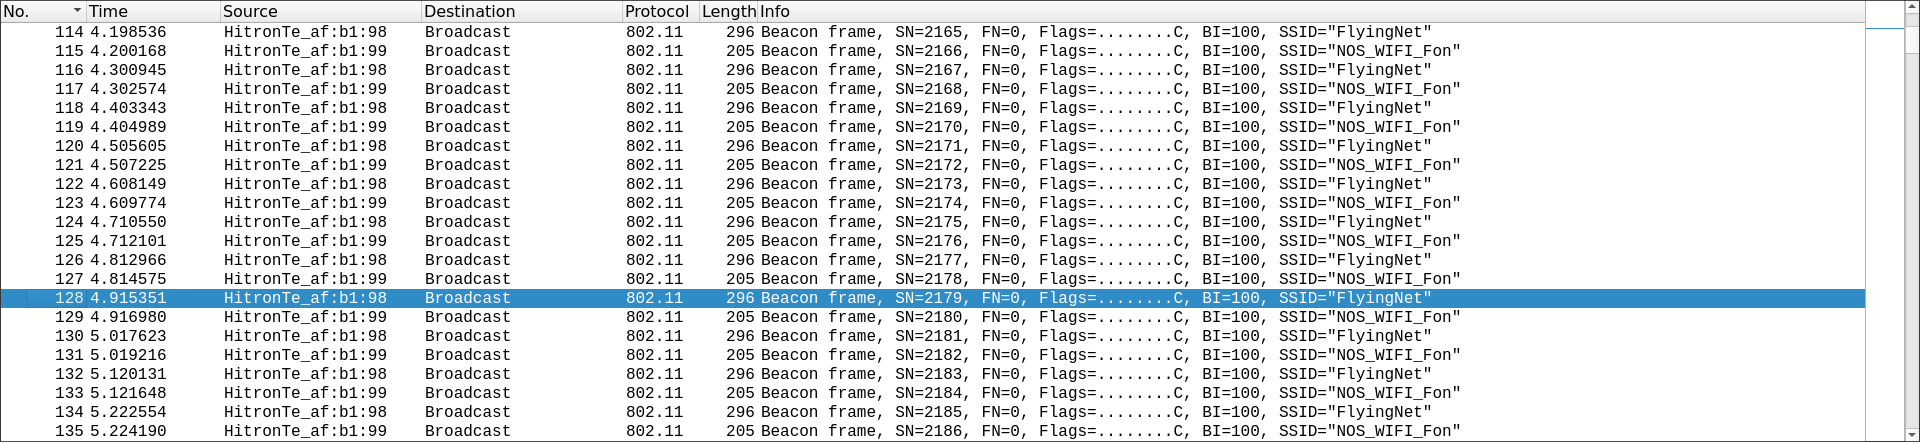
\includegraphics[width=0.8\textwidth]{images/ssids.png}
    \caption{\label{fig:ssids}SSIDs dos APs que estão a operar na vizinhança da STA de captura.}
\end{figure}

A lista dos SSIDs dos APs que estão a operar na vizinhança da STA de captura é a seguinte:
\begin{itemize}
    \item FlyingNet
    \item NOS\_WIFI\_Fon
\end{itemize}

\subsection{Face ao endereçamento usado, indique a que sistemas são endereçadas ambas as tramas e explique qual o propósito das mesmas?}

Quanto ao Probe Request, o Source Address é ea:a4:64:7b:b9:7a e o Destination Address é ff:ff:ff:ff:ff. Como o Probe Request é uma mensagem enviada por um dispositivo cliente Wi-Fi para explorar a presença de redes sem fio ao seu redor, o Destination Address é um Broadcast, de forma a reconhecer todos os APs presentes ao redor.
Quanto ao Probe Response, o Source Address é bc:14:01:af:b1:98 e o Destination Address é ea:a4:64:7b:b9:7a. A response tem como source o router, que manda o endereço MAC do AP que está enviando a resposta de sondagem, e tem como Destination o dispositivo que fez a request.

\begin{figure}[h]
    \centering
    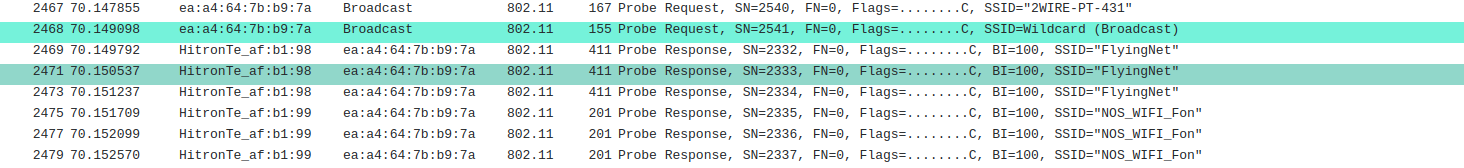
\includegraphics[width=0.8\textwidth]{images/responserequest.png}
    \caption{\label{fig:responserequest}Probes Requests e suas respectivas Probe Responses}
\end{figure}

\subsection*{Processo de Associação}

\subsection{Identifique uma sequência de tramas que corresponda a um processo de
associação completo entre a STA e o AP, incluindo a fase de autenticação.}

\begin{figure}[h]
    \centering
    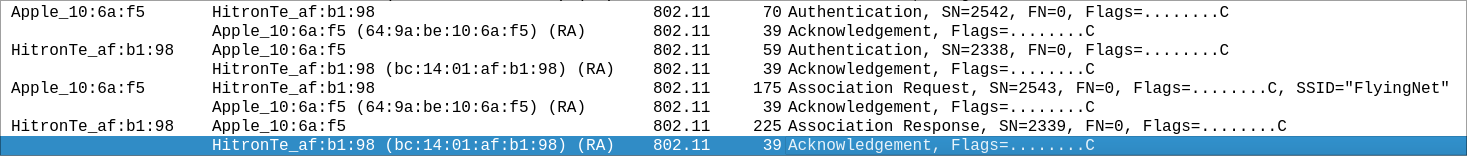
\includegraphics[width=0.8\textwidth]{images/association.png}
    \caption{\label{fig:association}Sequencia de tramas de processo de associacao}
\end{figure}

\subsection{Efetue um diagrama que ilustre, com as tramas identificadas na alínea anterior, a
sequência de todas as tramas trocadas no processo de autenticação e associação
entre o STA e o AP.}

Sequencia de tramas de processo de associacao:
\begin{itemize}
    \item \(STA \rightarrow AP: Authentication\ Request\)
    \item \(AP \rightarrow STA: Acknowledgment\)
    \item \(AP \rightarrow STA: Authentication\ Response\)
    \item \(STA \rightarrow AP: Acknowledgment\)
    \item \(STA \rightarrow AP: Association\ Request\)
    \item \(AP \rightarrow STA: Acknowledgment\)
    \item \(AP \rightarrow STA: Association\ Response\)
    \item \(STA \rightarrow AP: Acknowledgment\)
\end{itemize}

\subsection*{Transferência de Dados}

\subsection{Considere a trama de dados n.º 622. Sabendo que o campo Frame Control
contido no cabeçalho das tramas 802.11 permite especificar a direcionalidade
das tramas, o que pode concluir face à direcionalidade dessa trama? Será local à
WLAN?}

Podemos observar nas Flags do Frame Control, o campo DS status, que indica se a trama é destinada ao sistema de distribuição (DS) ou se vem do sistema de distribuição.
A trama possui (To DS: 0 From DS: 1), isso indica que a trama é enviada de um dispositivo cliente para o sistema de distribuição (como um AP). Ela é direcionada ao sistema de distribuição. A trama está se movendo do dispositivo cliente para o ponto de acesso, que é parte do sistema de distribuição da rede Wi-Fi. Portanto, essa trama é local à WLAN (Wireless Local Area Network) específica, ou seja, ela está sendo transmitida internamente na rede sem fio, de um dispositivo cliente para o ponto de acesso que faz parte da mesma WLAN.

\subsection{Para a trama de dados da alínea anterior, transcreva os endereços MAC em uso,
identificando qual o endereço MAC correspondente ao host sem fios (STA), ao AP
e ao router de acesso ao sistema de distribuição.}

\begin{itemize}
    \item Source Address: bc:14:01:af:b1:96
    \item Destination Address: 64:9a:be:10:6a:f5
\end{itemize}

Como o source address é bc:14:01:af:b1:96, o MAC address do host sem fios (STA) é bc:14:01:af:b1:96. Já o MAC address correspondente ao AP é 64:9a:be:10:6a:f5, que é o destination address. O router de acesso ao sistema de distribuição é o endereço do AP que atua como como gateway para a rede com fio (Sistema de Distribuição), portanto, o seu MAC address também é 64:9a:be:10:6a:f5.

\subsection{Observa-se que ao longo da transferência de dados são usadas tramas de
controlo ACK. Tente explicar porque razão têm de existir, contrariamente ao que
acontece numa rede Ethernet.}

As tramas de controlo ACK são usadas para confirmar a receção de uma trama de dados, e para indicar que a estação está pronta para receber a próxima trama de dados.
Na rede Ethernet, as tramas de controlo ACK não são necessárias, pois a rede Ethernet é uma rede com fios, e por isso a probabilidade de perda de tramas de dados e menor, assim como a probabilidade de interferencias.

\subsection{Dê um exemplo de uma transferência de dados em que é usada a opção RTC/CTS
e um outro em que não é usada, identificando a direccionalidade das tramas, as
tramas de controlo e os sistemas envolvidos. Apresente as tramas e os sistemas
devidamente identificados sob a forma de um diagrama de sequência.}

De forma a filtrar os pacotes RTC/CTS foi utilizado o filtro no wireshark: \(wlan.fc.type\_subtype == 27\), foi selecionado um dos pacotes de rtc e dps o filtro foi removido de forma a ver todos os pacotes adjacentes.

\begin{figure}[h]
    \centering
    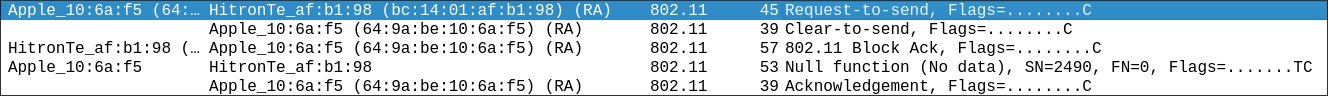
\includegraphics[width=0.8\textwidth]{images/rct.png}
    \caption{\label{fig:rct}Sequencia de tramas de RCT/CTS}
\end{figure}

\begin{itemize}
    \item \(STA \rightarrow AP: Request\ to\ Send\)
    \item \(AP \rightarrow STA: Clear\ to\ Send\)
    \item \(STA \rightarrow AP: Null\ function\)
    \item \(AP \rightarrow STA: Acknowledgment\)
\end{itemize}

\section{Conclusao}

Neste relatório, exploramos com sucesso dois aspectos fundamentais de sistemas de redes: o Protocolo ARP e a tecnologia Wi-Fi IEEE 802.11. No que toca ao ARP, adquirimos uma compreensão sólida de como as tabelas de endereçamento são usadas para mapear endereços IP a endereços MAC, e como esse processo é essencial para o funcionamento de redes locais. Além disso, ao examinar a integração de novos dispositivos em redes domésticas, identificamos as complexidades envolvidas na resolução de endereços e na descoberta de dispositivos.

Em relação ao IEEE 802.11, exploramos os sistemas de Controle de Acesso ao Meio (MAC) e técnicas como o RTS/CTS (Request to Send/Clear to Send) para aprimorar a eficiência da transmissão de pacotes em redes Wi-Fi. Compreendemos que a otimização do acesso ao meio é crucial para manter o desempenho e a confiabilidade das redes sem fio, especialmente em ambientes com vários dispositivos.

Esse trabalho proporcionou-nos insights valiosos sobre a operação interna das redes, tornando-nos mais conscientes dos desafios e soluções relacionados à conectividade. À medida que continuamos a avançar no estudo de sistemas de redes, estamos confiantes de que esse conhecimento enriquecerá as nossas habilidades e contribuirá para a construção e manutenção eficazes de infraestruturas de comunicação de dados.


\end{document}